\documentclass{beamer}
\usepackage[T1]{fontenc}
\usepackage[english]{babel}
\usepackage{lmodern}
\usepackage{amsmath,amssymb}
\usepackage{algorithm}
\usepackage{algorithmic}
\usepackage{graphicx}
\usepackage{subcaption}
\usepackage{caption}
\usepackage{tikz}
\usetikzlibrary{overlay-beamer-styles}
\usepackage{booktabs,multicol,stackengine}
\usepackage[table,dvipsnames]{xcolor}
\usepackage{cancel}
\usepackage{moresize}

\usepackage{hyperref}

\usepackage{listings}
\definecolor{nus-orange}{RGB}{239,124,0}
\definecolor{nus-blue}{RGB}{0,61,124}
\definecolor{halfgray}{gray}{0.55}

\lstset{
  basicstyle=\ttfamily\footnotesize,
  keywordstyle=\bfseries\color{nus-blue},
  stringstyle=\color{ForestGreen},
  numbers=left,
  numberstyle=\scriptsize\color{halfgray},
  rulesepcolor=\color{nus-orange},
  frame=shadowbox,
  columns=flexible,
  showstringspaces=false,
  keepspaces=true,
  tabsize=2,
  breaklines=true
}

\renewcommand{\figurename}{Figure}
\renewcommand{\algorithmname}{Algorithm}

\usepackage{SHU}
\input{macros}

\title{BT5110: Tutorial 2 — Entity - Relationship Model}
\author{\href{https://pratik2358.github.io/}{Pratik Karmakar}}
\institute{School of Computing,\\ National University of Singapore}
\date{AY26/27 S1}

\begin{document}
\begin{frame}
  \titlepage
  \IfFileExists{nus-logo.png}{
    \begin{figure}[htpb]\centering
      
\includegraphics[keepaspectratio, scale=0.18]{nus-logo.png}
    \end{figure}
  }{}
\end{frame}

\begin{frame}{The Problem}
\tiny
The Varsity International Network of Oenology wishes to computerise the management of the information about its members as well as to record the information they gather about various wines. Your company, Apasaja Private Limited, is commissioned by the Varsity International Network of Oenology to design and implement the relational schema of the database application. The organisation is big enough so that there could be several members with the same name. A card with a unique number is issued to identify each drinker. The contact address of each member is also recorded for the mailing of announcements and calls for meetings.

At most once a week, VINO organises a tasting session. At each session, the attending members taste several bottles. Each member records for each bottle his or her evaluation of the quality (very good, good, average, mediocre, bad, very bad) of each wine that she or he tastes. The evaluation may differ for the same wine from one drinker to another. Actual quality and therefore evaluation also varies from one to another bottle of a given wine. Every bottle that is opened during the tasting session is finished during that session.

Each wine is identified by its name (“Parade D'Amour”), appellation (“Bordeaux”) and vintage (1990). Other information of interest about the wine is the degree of alcohol (11.5), where and by whom it has been bottled (“Mis en Bouteille par Amblard-Larolphie Negociant-Eleveur a Saint Andre de Cubzac (Gironde) - France”), the certification of its appellation if available (“Appellation Bordeaux Controlée”), and the country it comes from (produce of “France”).

Generally, there are or have been several bottles of the same wine in the cellar. For each wine, the bottles in the wine cellar of VINO are numbered. For instance, the cellar has 20 bottles numbered 1 to 20 of a Semillon from 1996 named Rumbalara. For documentation purposes, VINO may also want to record wines for which it does not own bottles. The bottles are either available in the cellar or they have been tasted and emptied.

We first want to design an entity-relationship schema that most correctly and most completely captures the constraints expressed in the above description of the VINO application.

\end{frame}

\begin{frame}
    \begin{figure}
        \centering
        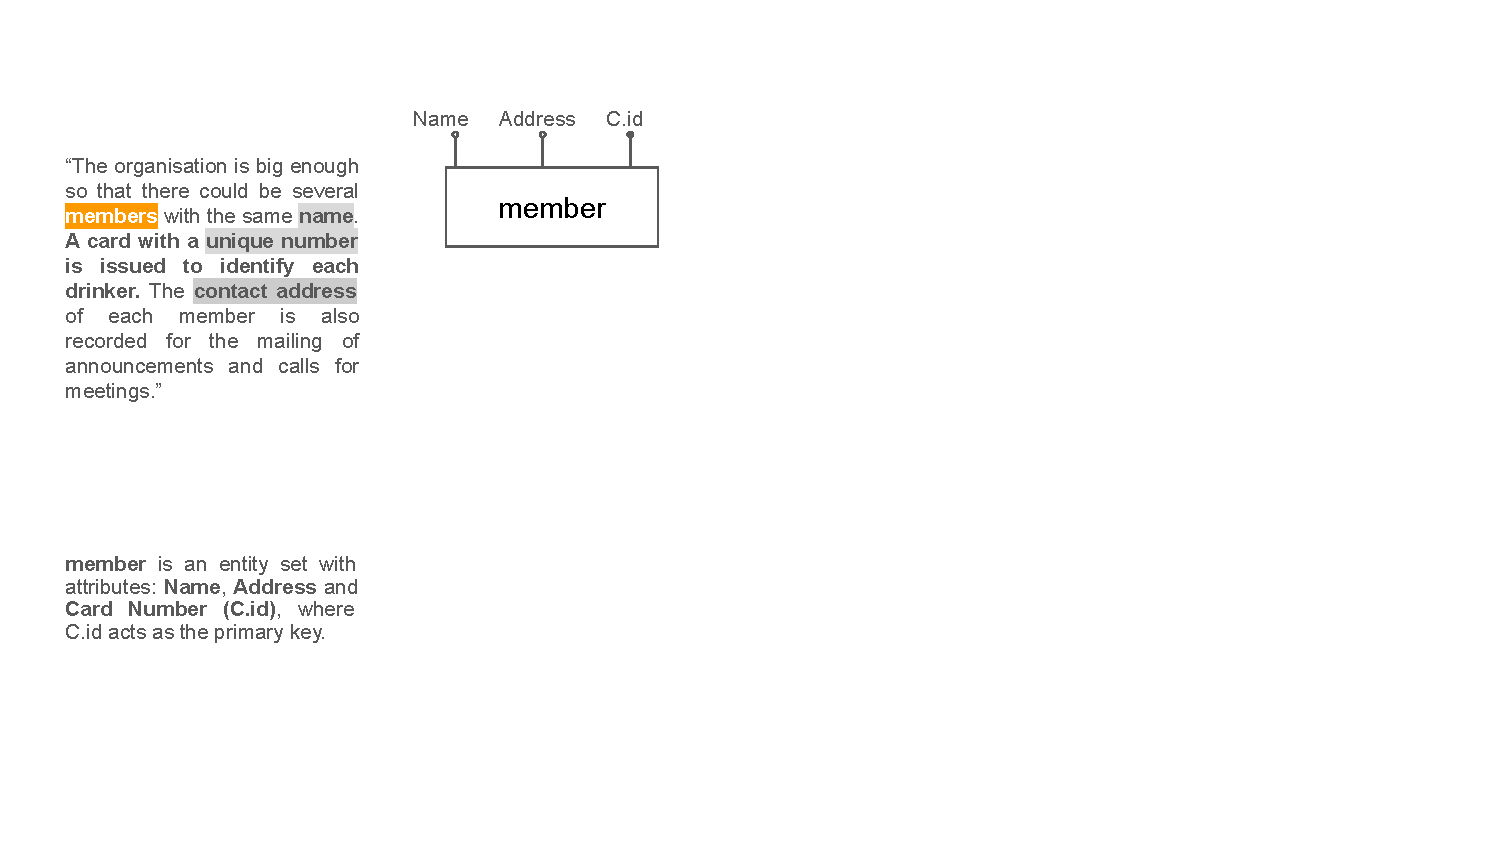
\includegraphics[width=1.1\linewidth]{tut_02_files/01.pdf}
    \end{figure}
\end{frame}

\begin{frame}
    \begin{figure}
        \centering
        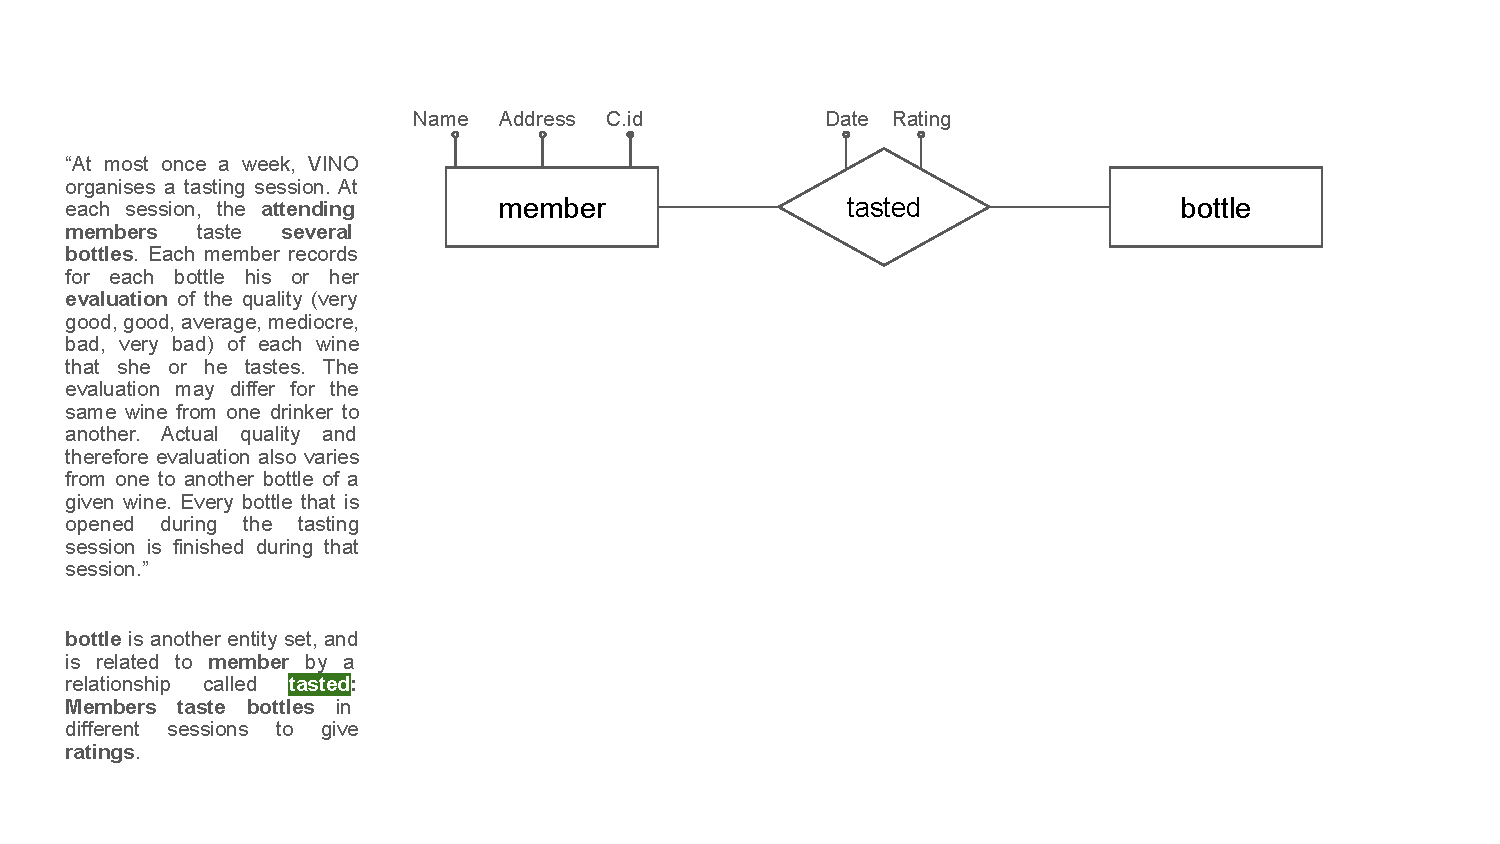
\includegraphics[width=1.1\linewidth]{tut_02_files/02.pdf}
    \end{figure}
\end{frame}

\begin{frame}
    \begin{figure}
        \centering
        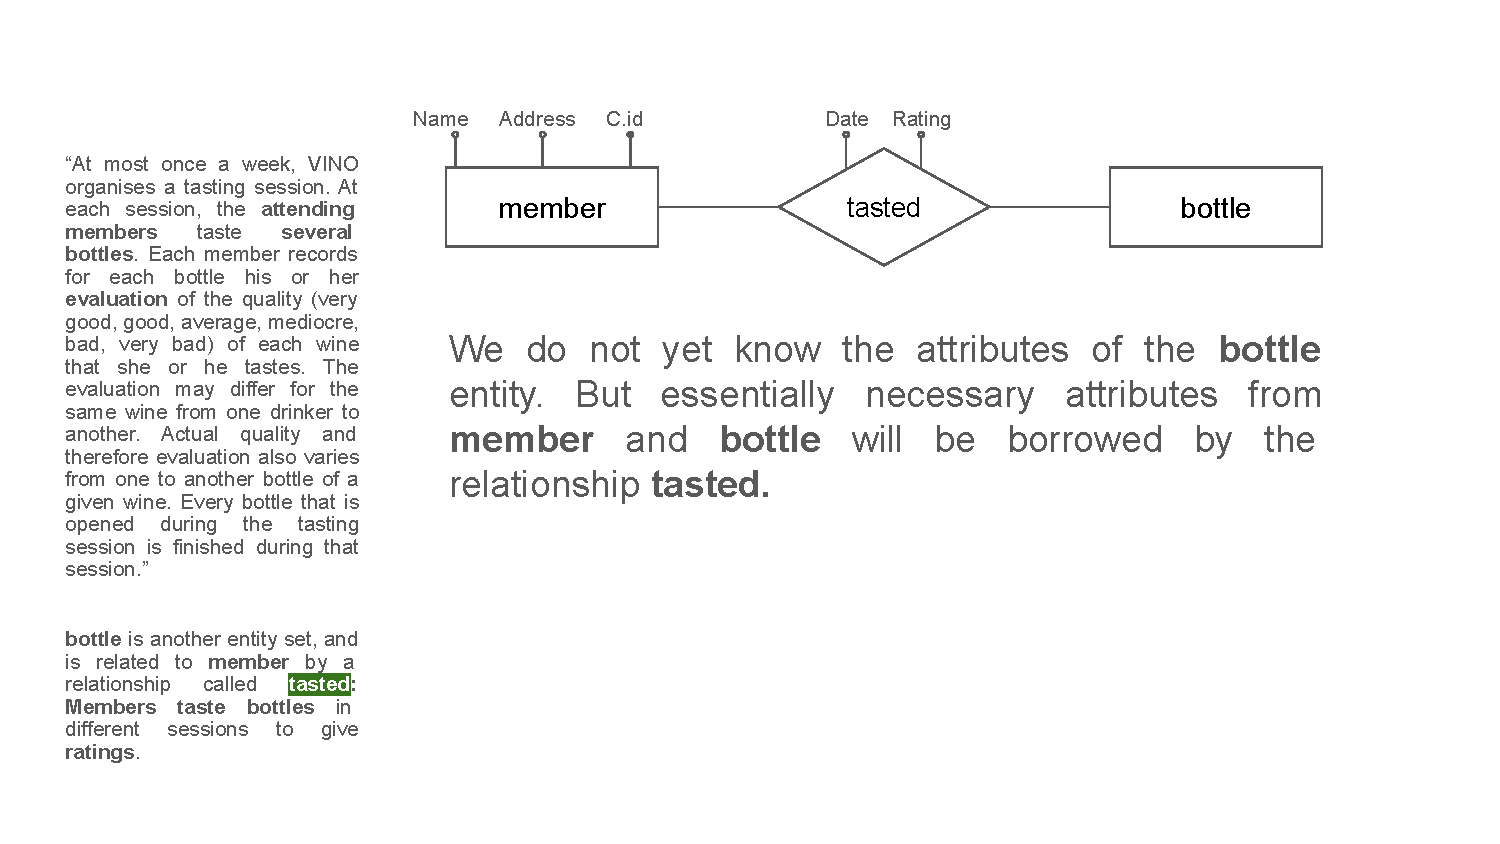
\includegraphics[width=1.1\linewidth]{tut_02_files/03.pdf}
    \end{figure}
\end{frame}

\begin{frame}
    \begin{figure}
        \centering
        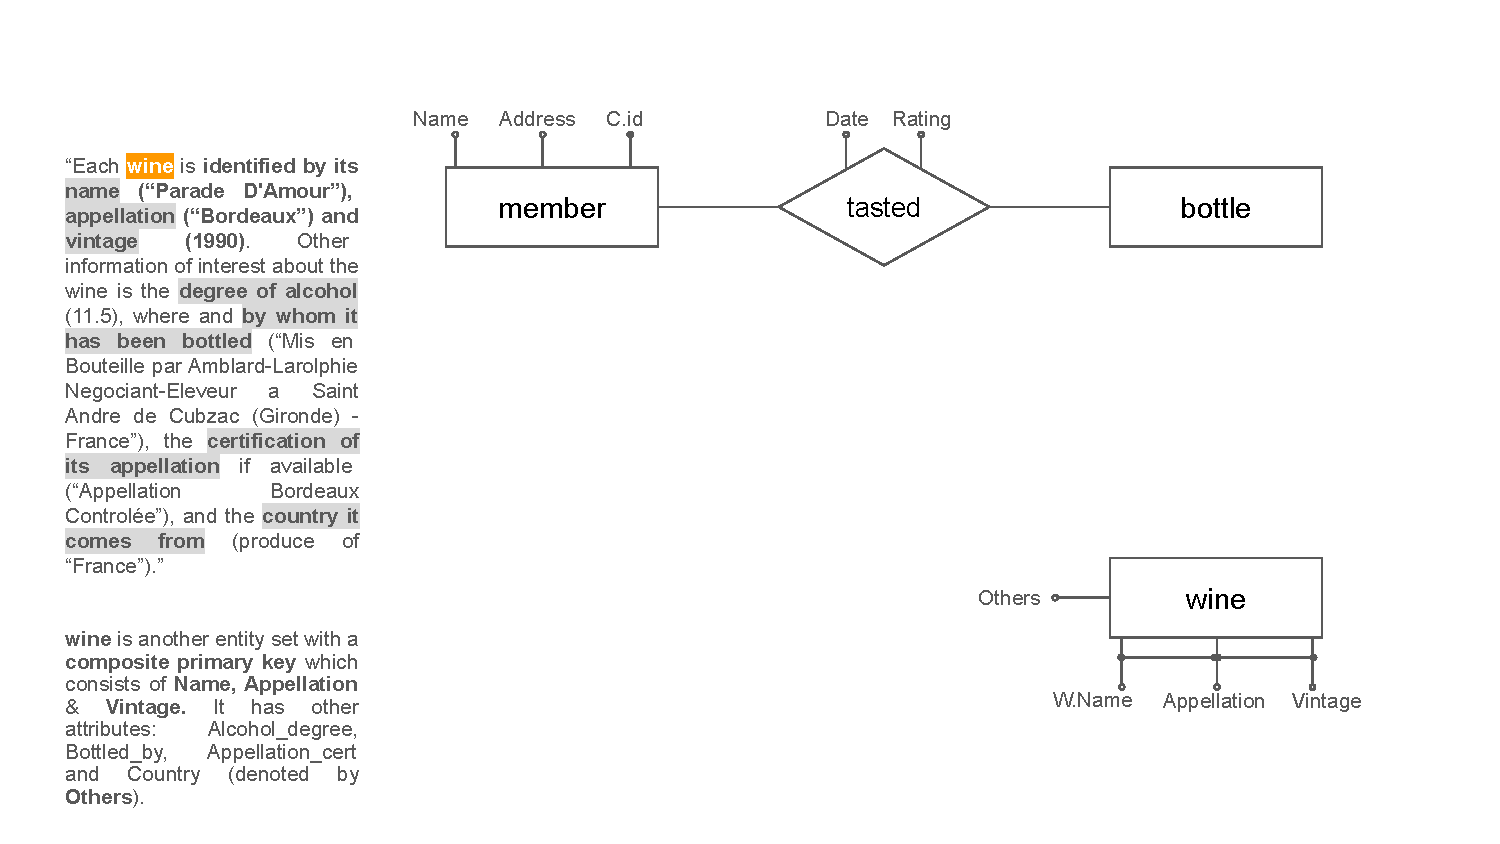
\includegraphics[width=1.1\linewidth]{tut_02_files/04.pdf}
    \end{figure}
\end{frame}

\begin{frame}
    \begin{figure}
        \centering
        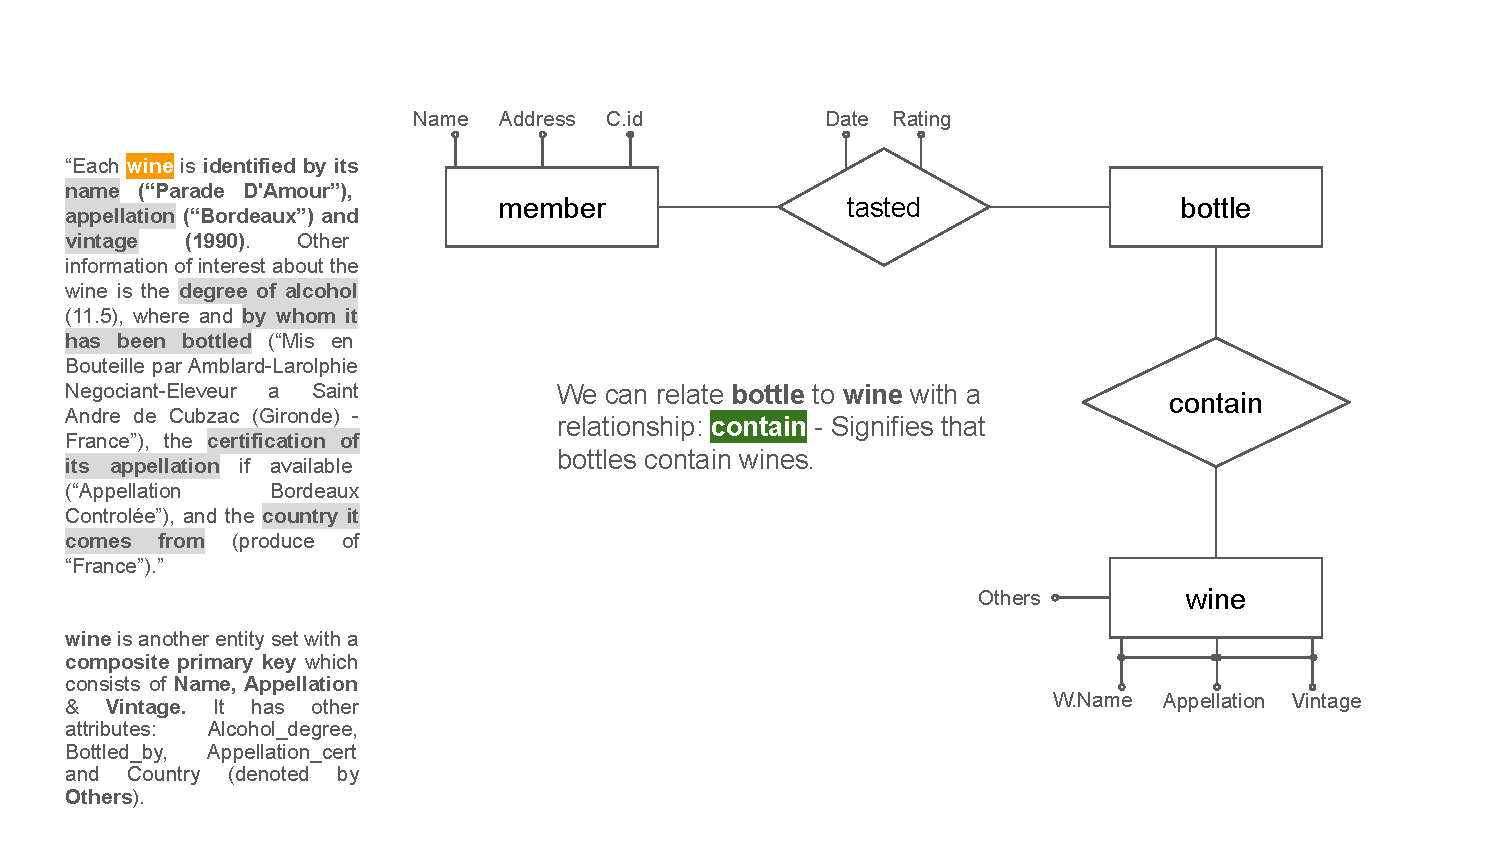
\includegraphics[width=1.1\linewidth]{tut_02_files/05.pdf}
    \end{figure}
\end{frame}

\begin{frame}
    \begin{figure}
        \centering
        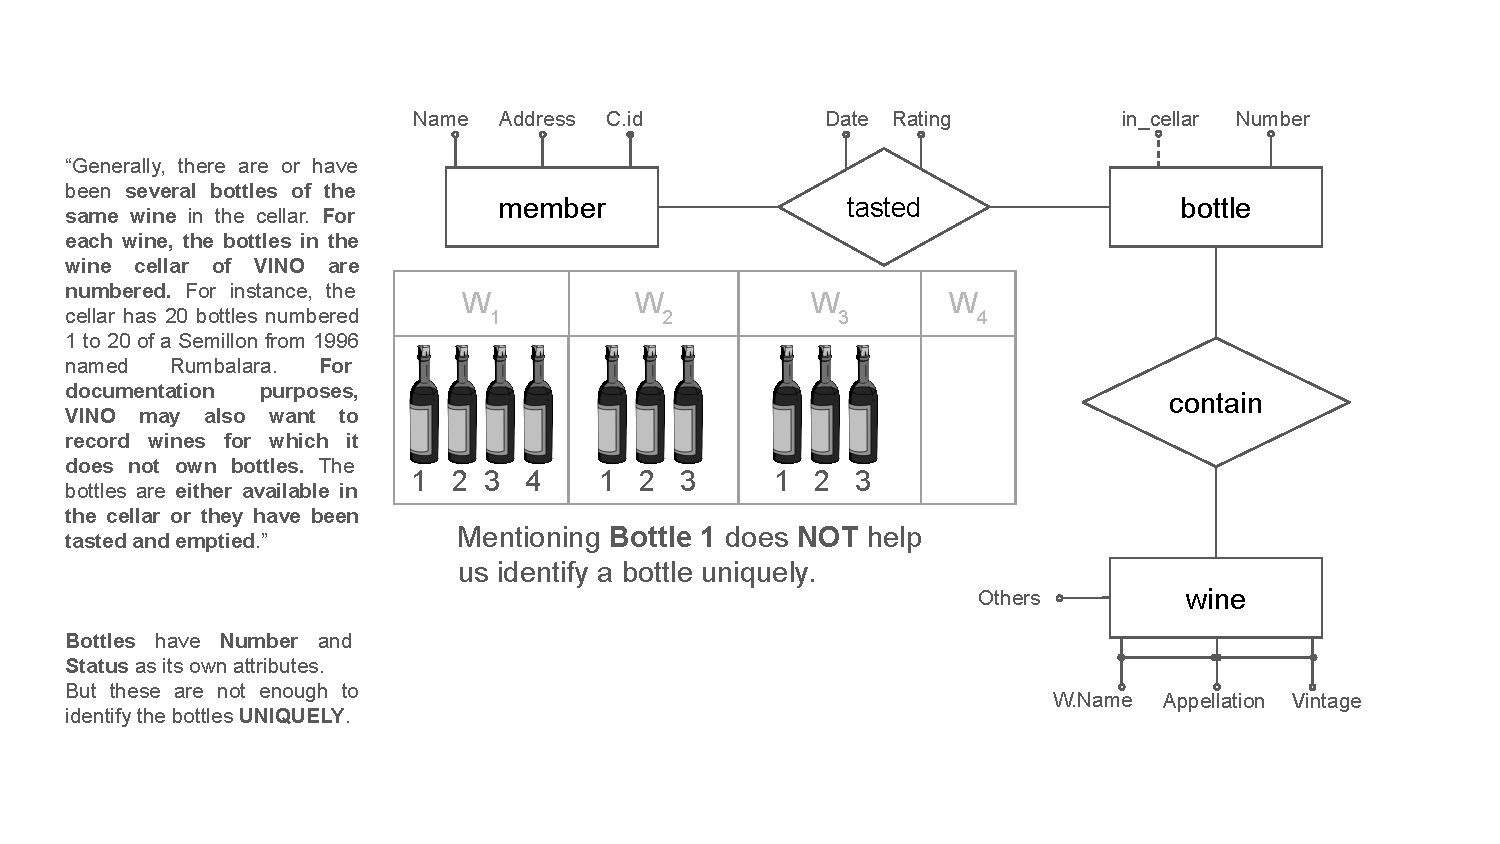
\includegraphics[width=1.1\linewidth]{tut_02_files/06.pdf}
    \end{figure}
\end{frame}

\begin{frame}
    \begin{figure}
        \centering
        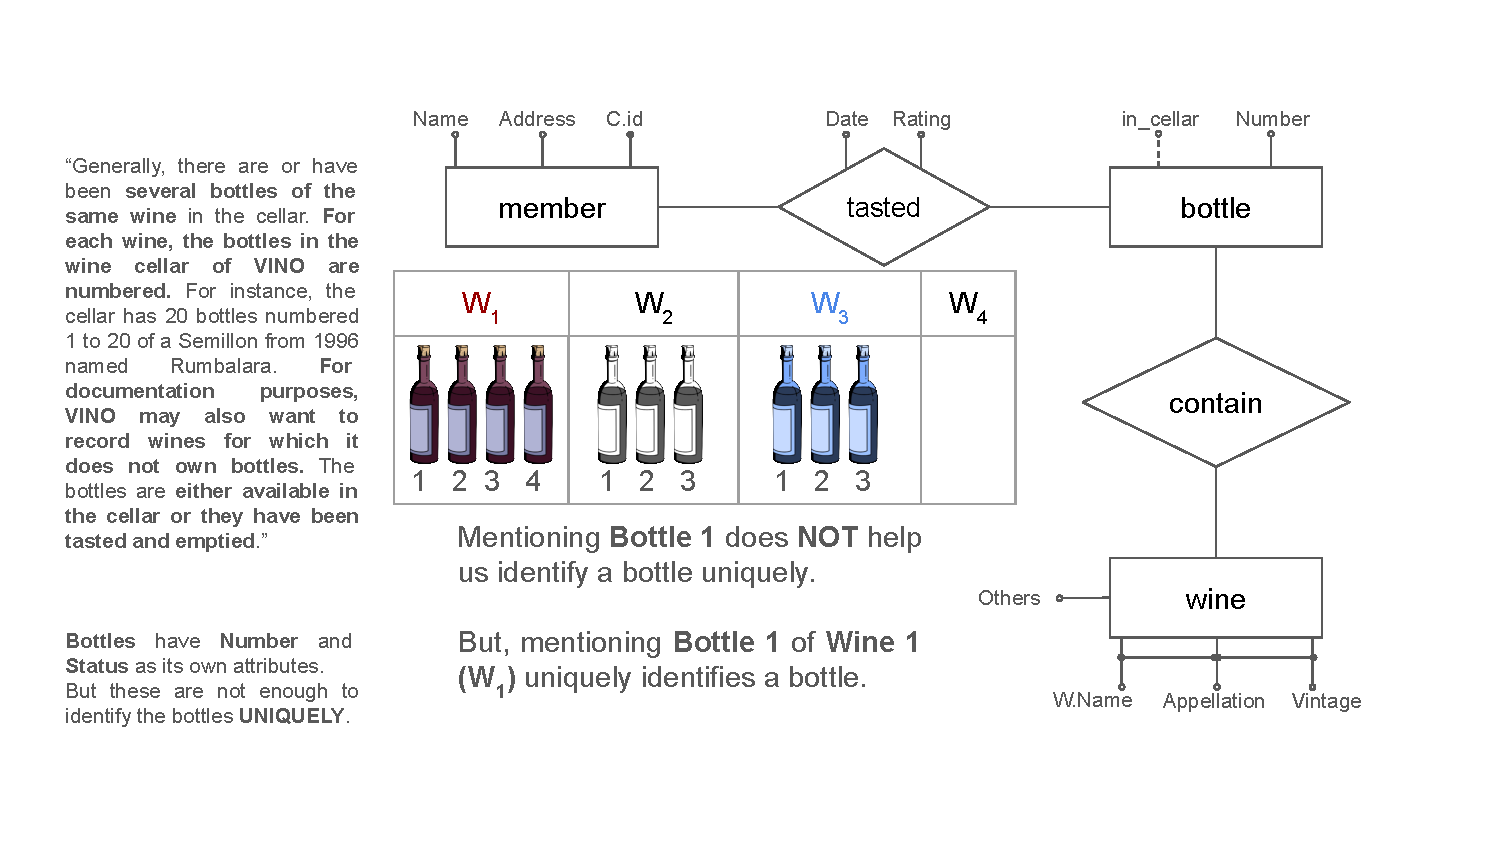
\includegraphics[width=1.1\linewidth]{tut_02_files/07.pdf}
    \end{figure}
\end{frame}

\begin{frame}
    \begin{figure}
        \centering
        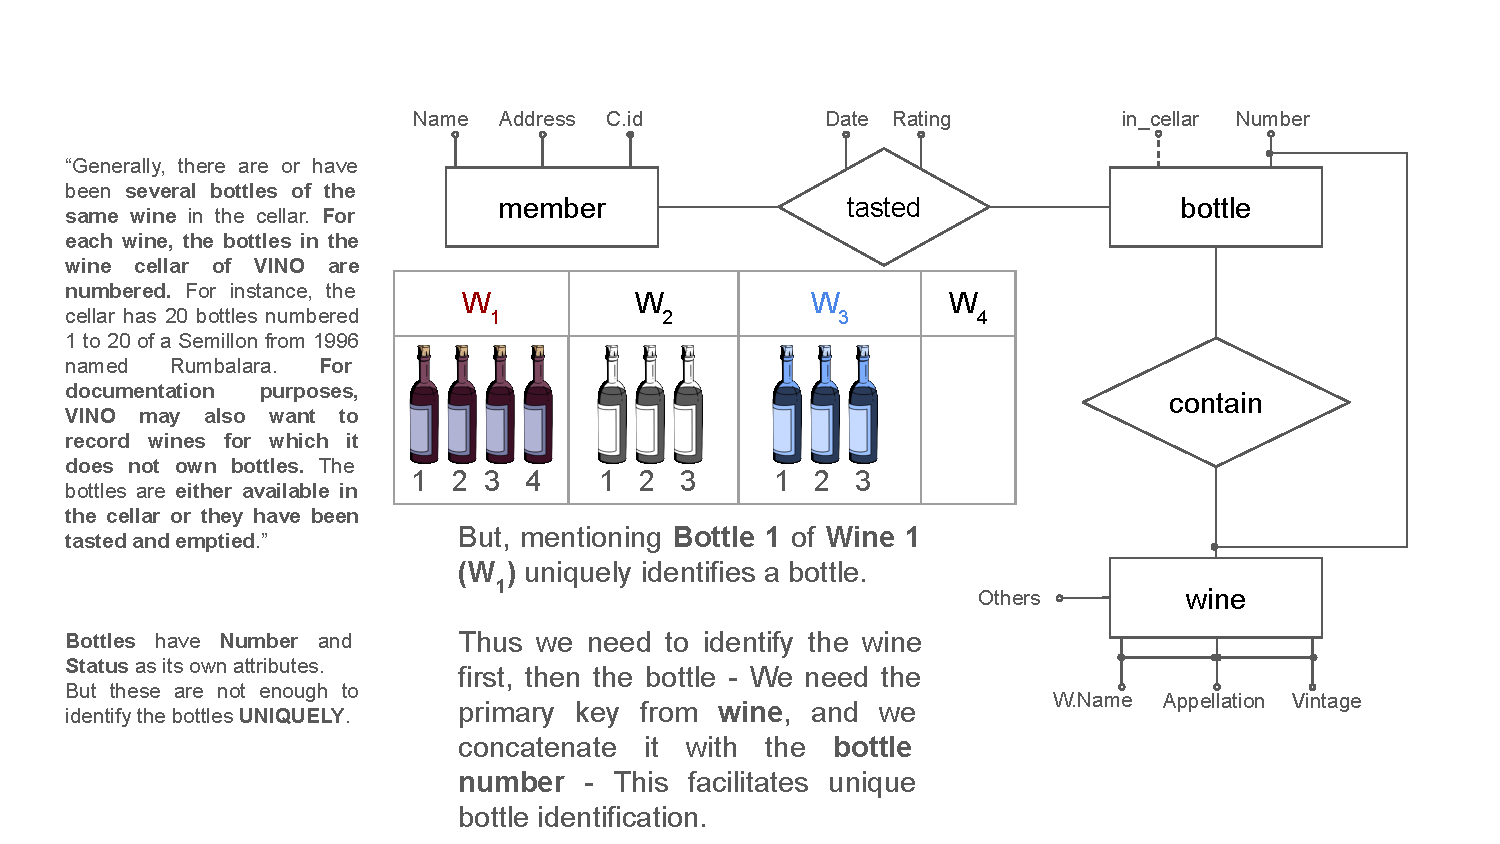
\includegraphics[width=1.1\linewidth]{tut_02_files/08.pdf}
    \end{figure}
\end{frame}

\begin{frame}
    \begin{figure}
        \centering
        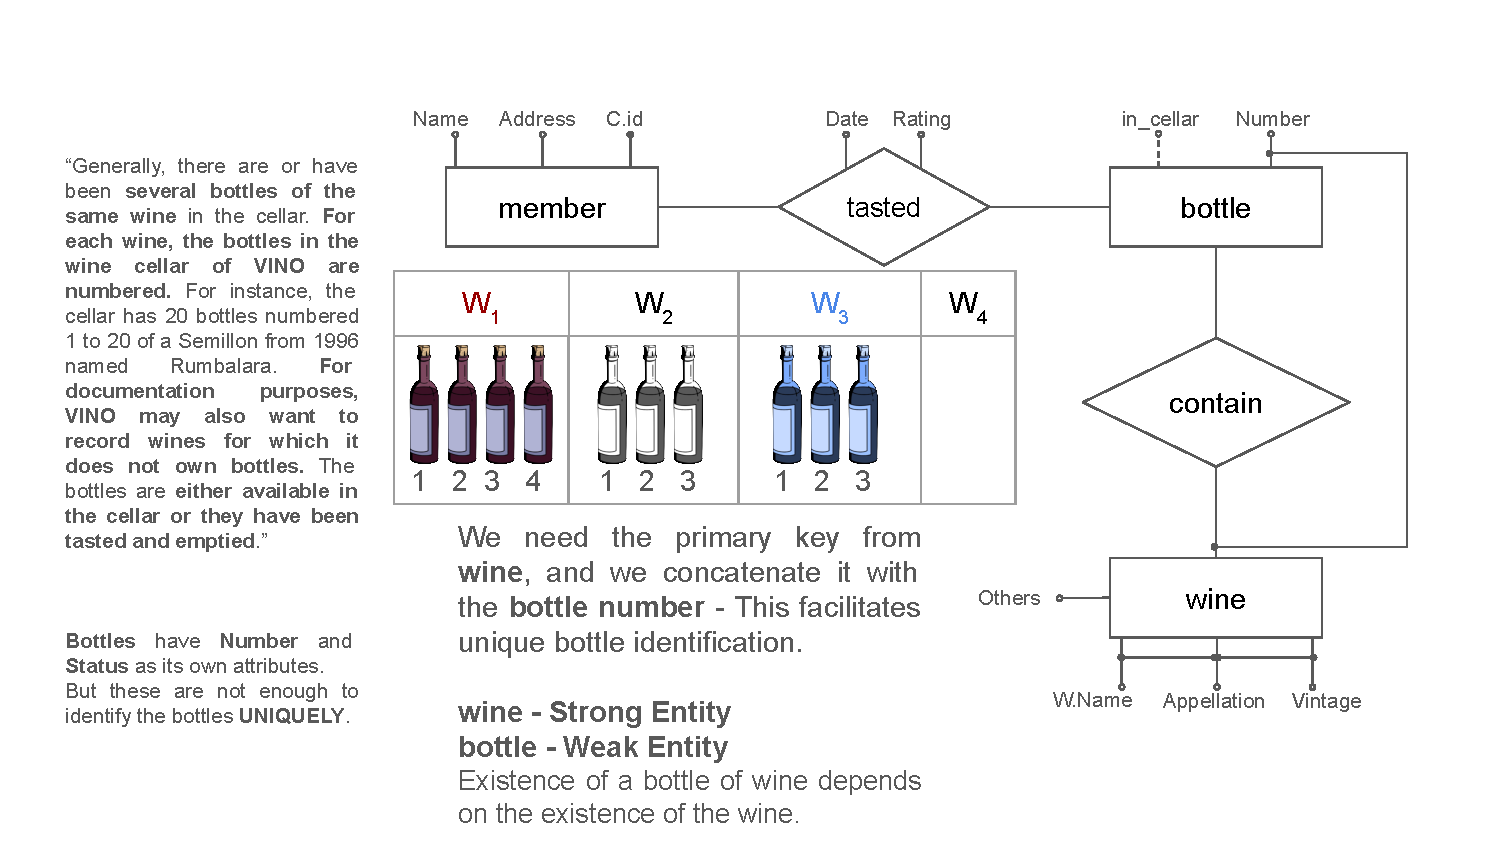
\includegraphics[width=1.1\linewidth]{tut_02_files/09.pdf}
    \end{figure}
\end{frame}

\begin{frame}
    \begin{figure}
        \centering
        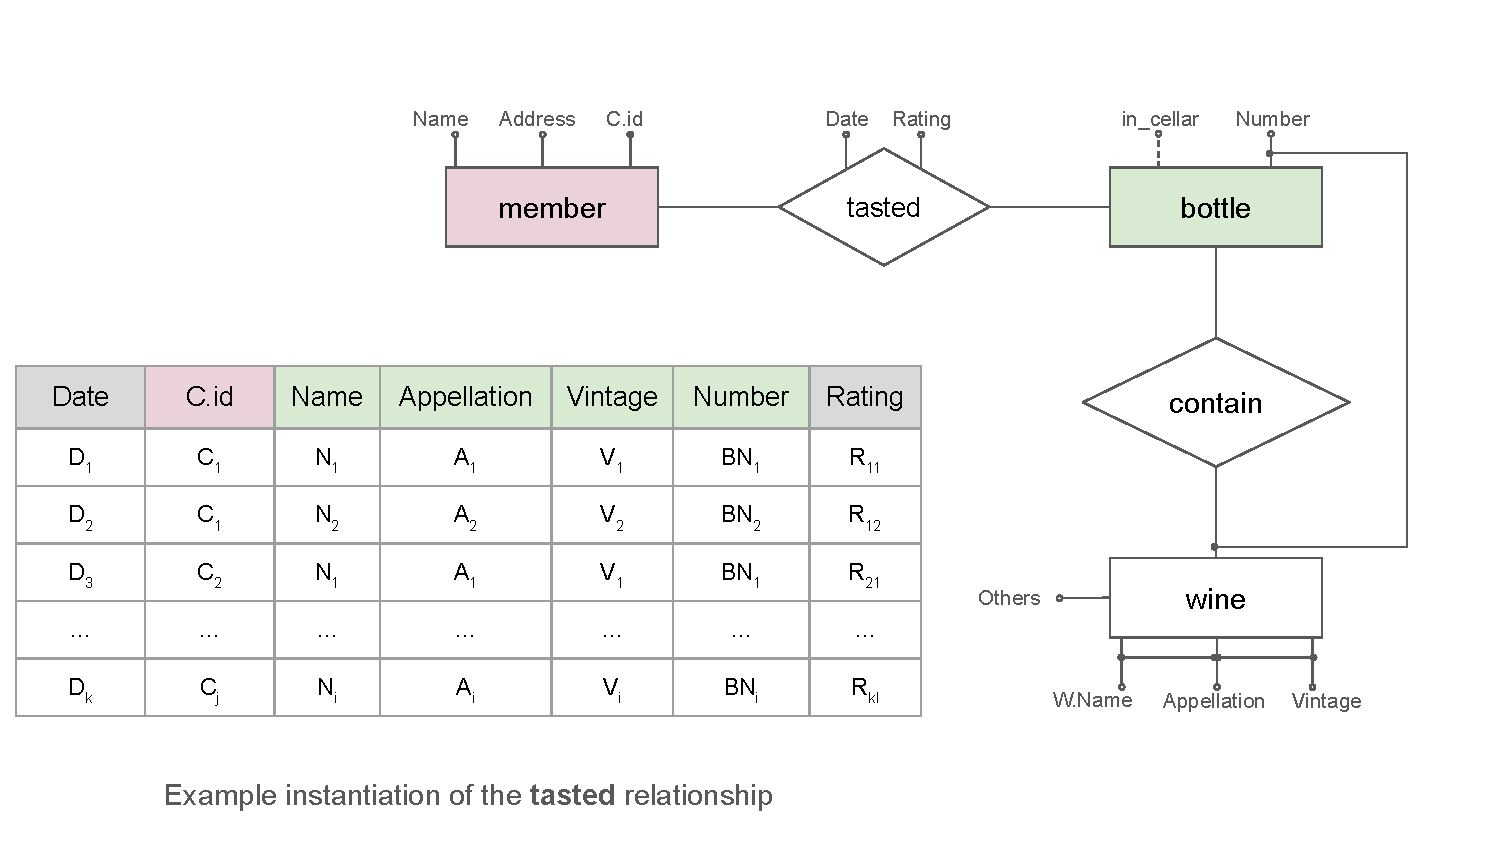
\includegraphics[width=1.1\linewidth]{tut_02_files/10.pdf}
    \end{figure}
\end{frame}

\begin{frame}
    \begin{figure}
        \centering
        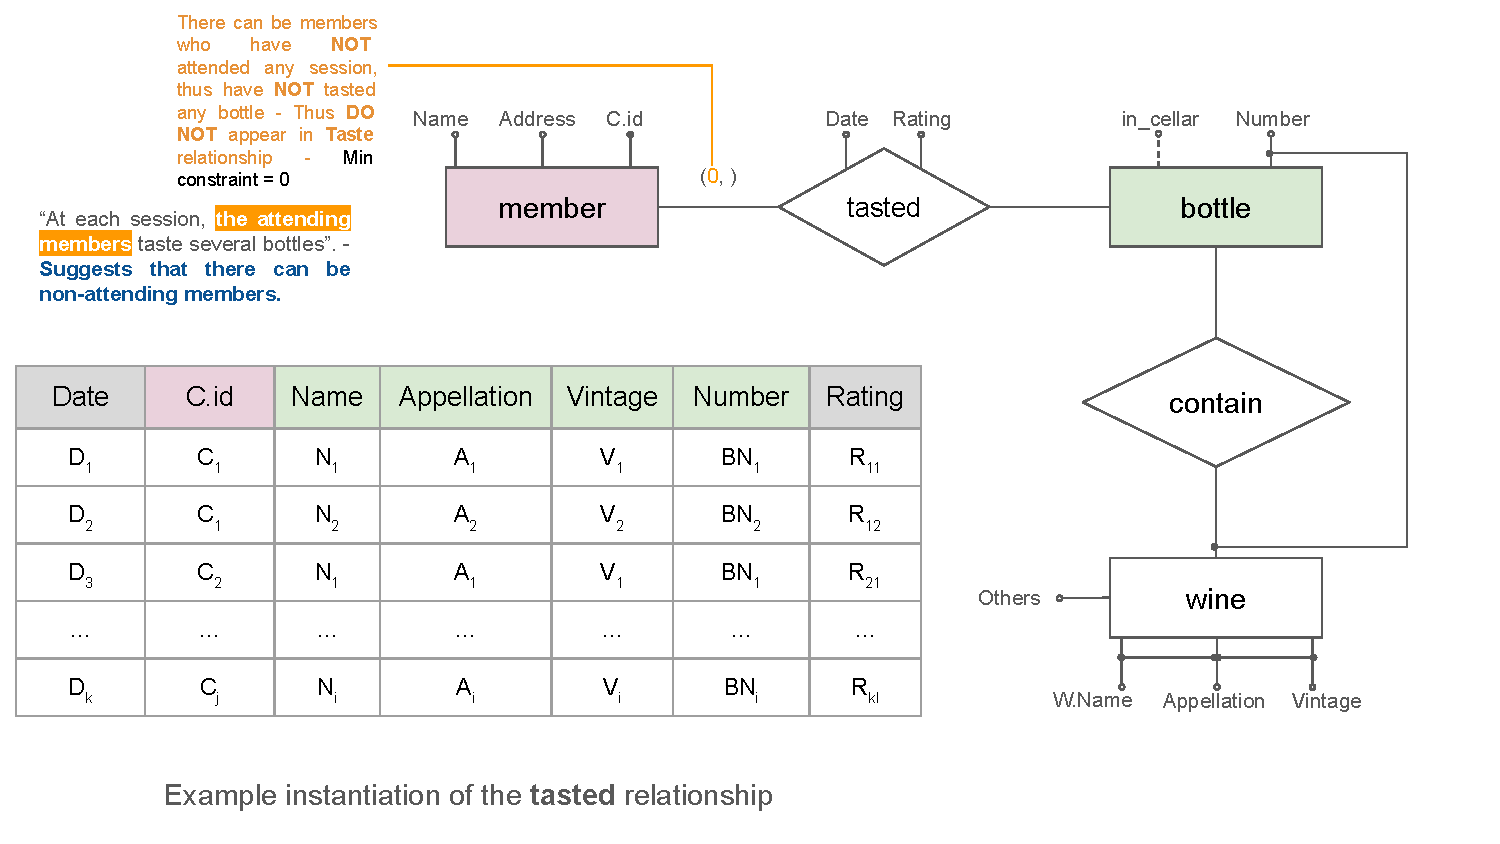
\includegraphics[width=1.1\linewidth]{tut_02_files/11.pdf}
    \end{figure}
\end{frame}

\begin{frame}
    \begin{figure}
        \centering
        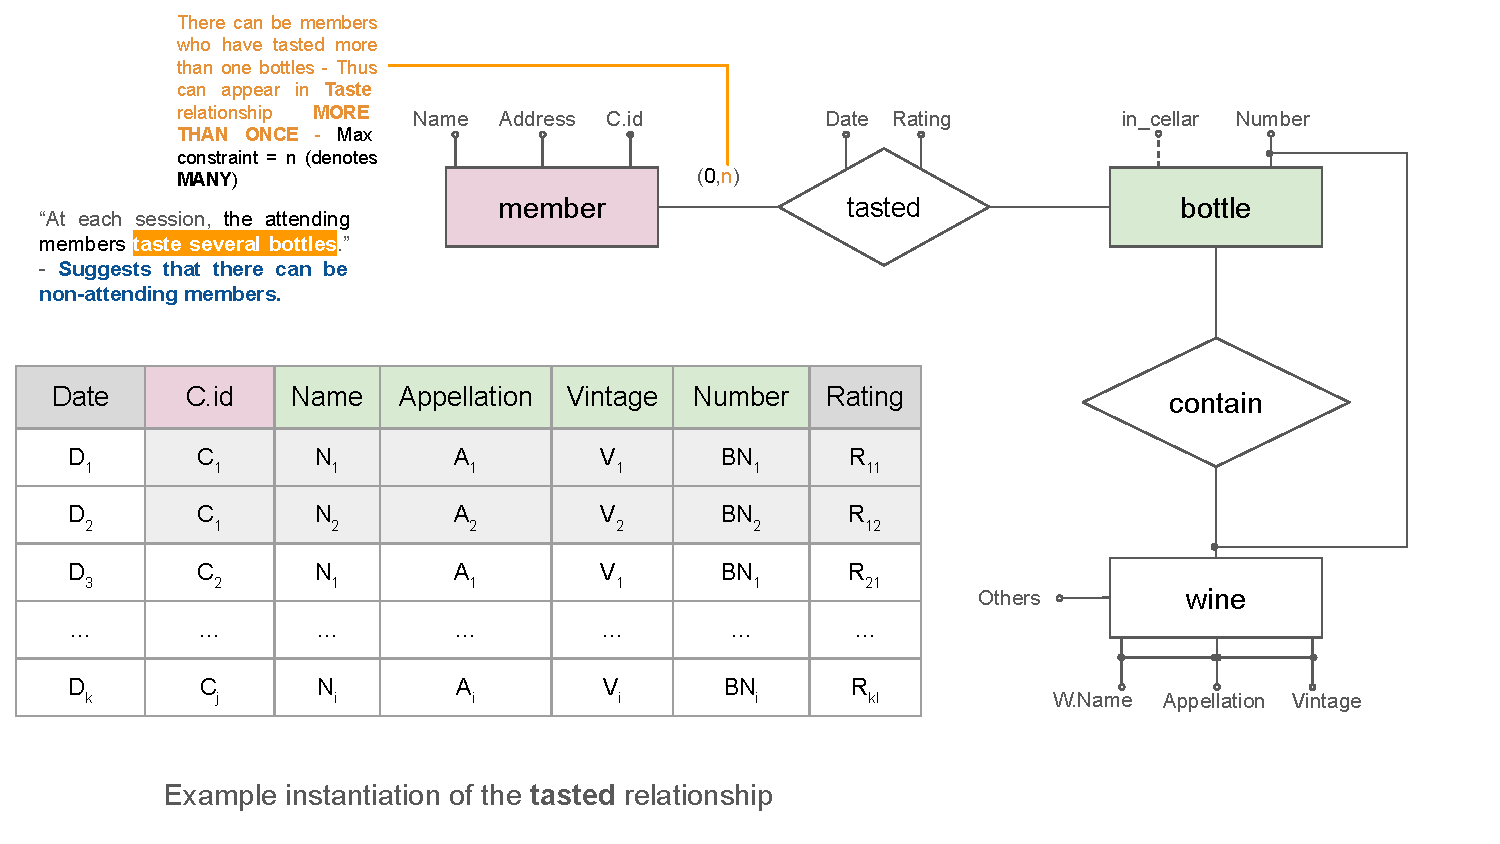
\includegraphics[width=1.1\linewidth]{tut_02_files/12.pdf}
    \end{figure}
\end{frame}

\begin{frame}
    \begin{figure}
        \centering
        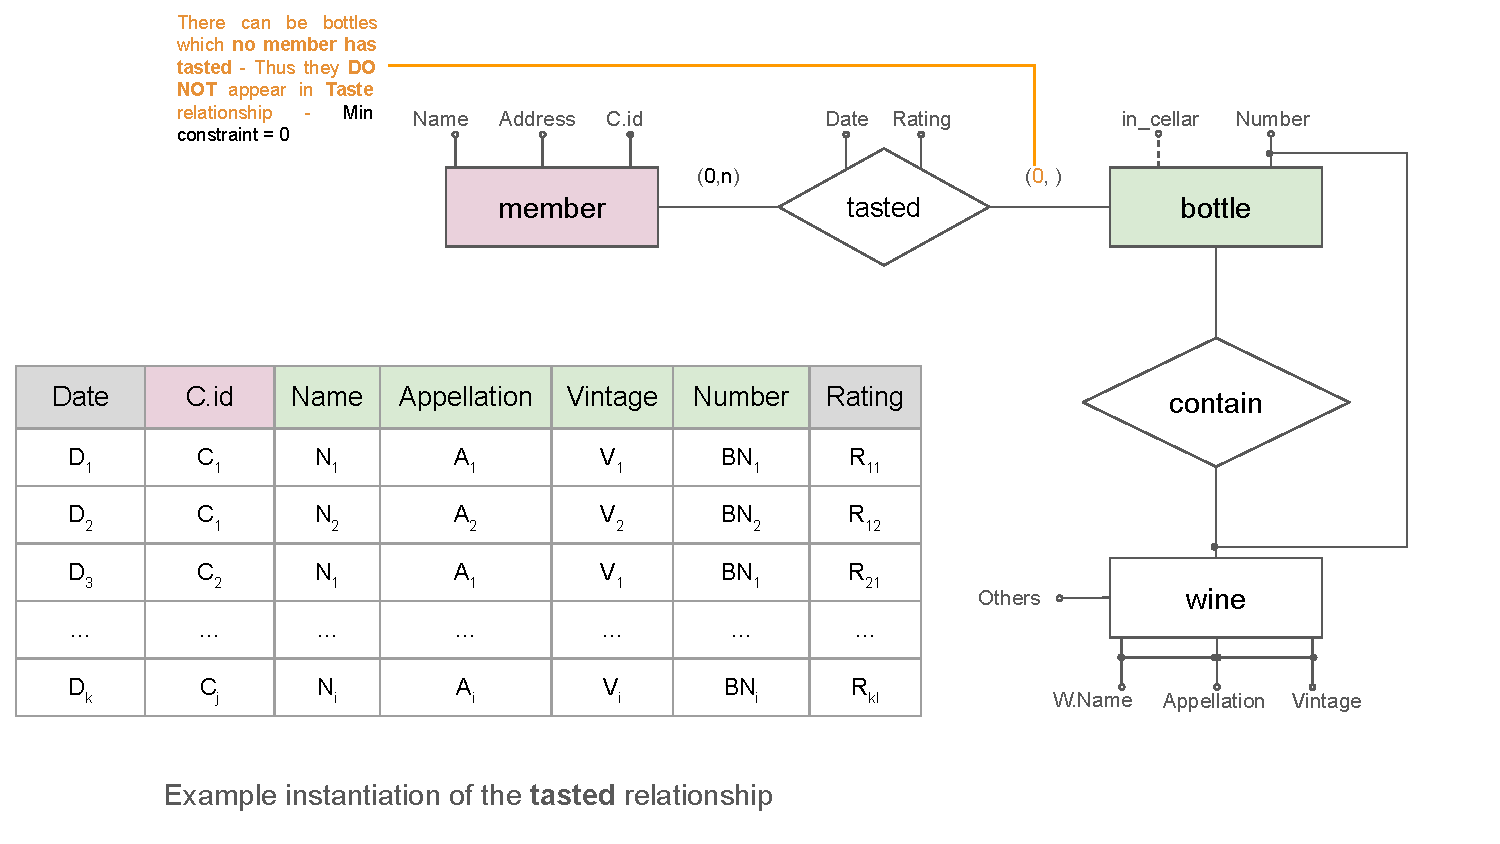
\includegraphics[width=1.1\linewidth]{tut_02_files/13.pdf}
    \end{figure}
\end{frame}

\begin{frame}
    \begin{figure}
        \centering
        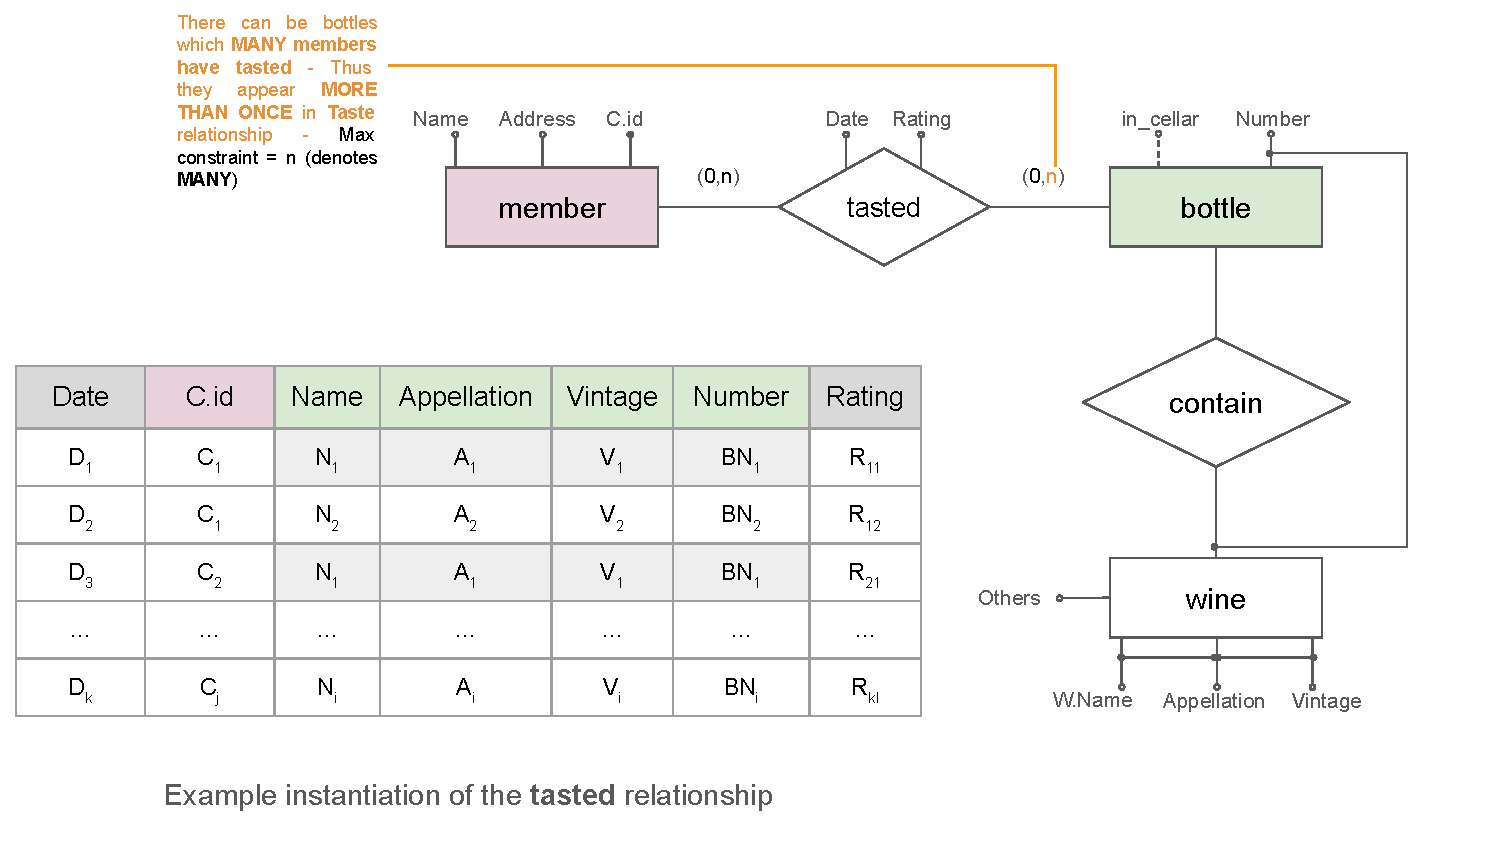
\includegraphics[width=1.1\linewidth]{tut_02_files/14.pdf}
    \end{figure}
\end{frame}

\begin{frame}
    \begin{figure}
        \centering
        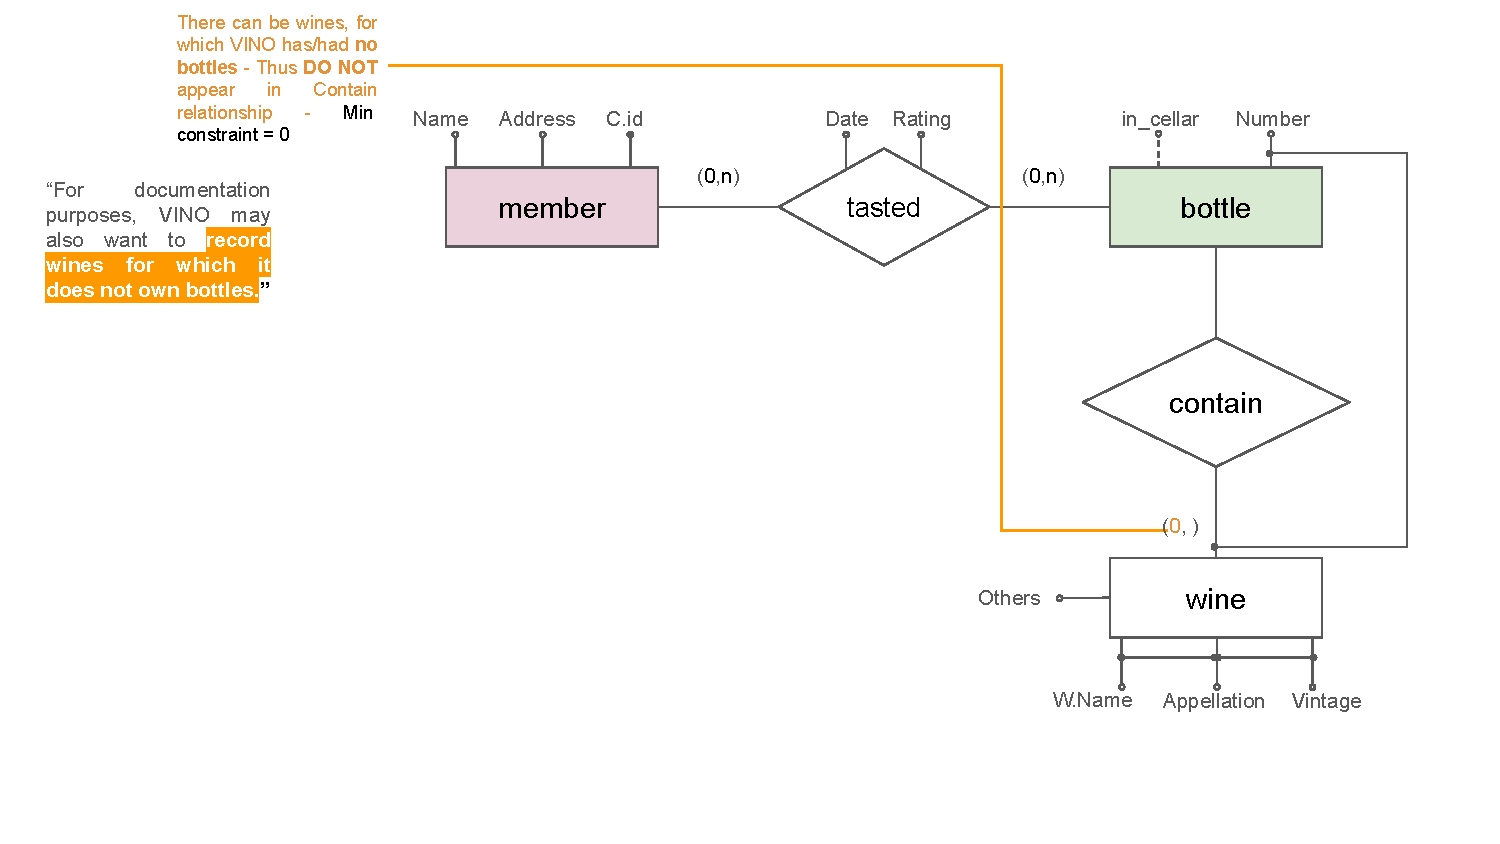
\includegraphics[width=1.1\linewidth]{tut_02_files/15.pdf}
    \end{figure}
\end{frame}

\begin{frame}
    \begin{figure}
        \centering
        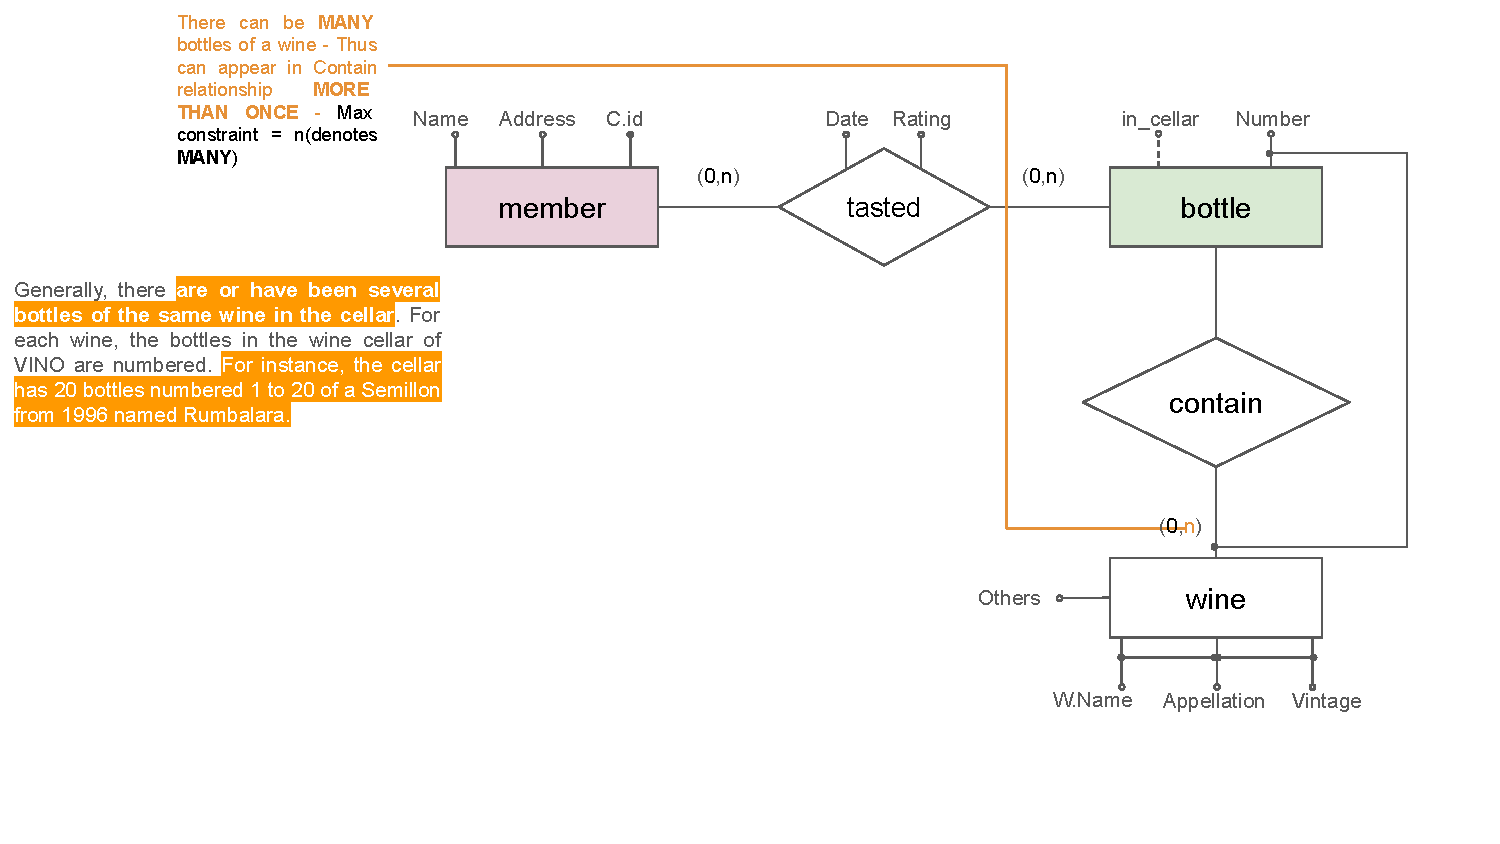
\includegraphics[width=1.1\linewidth]{tut_02_files/16.pdf}
    \end{figure}
\end{frame}

\begin{frame}
    \begin{figure}
        \centering
        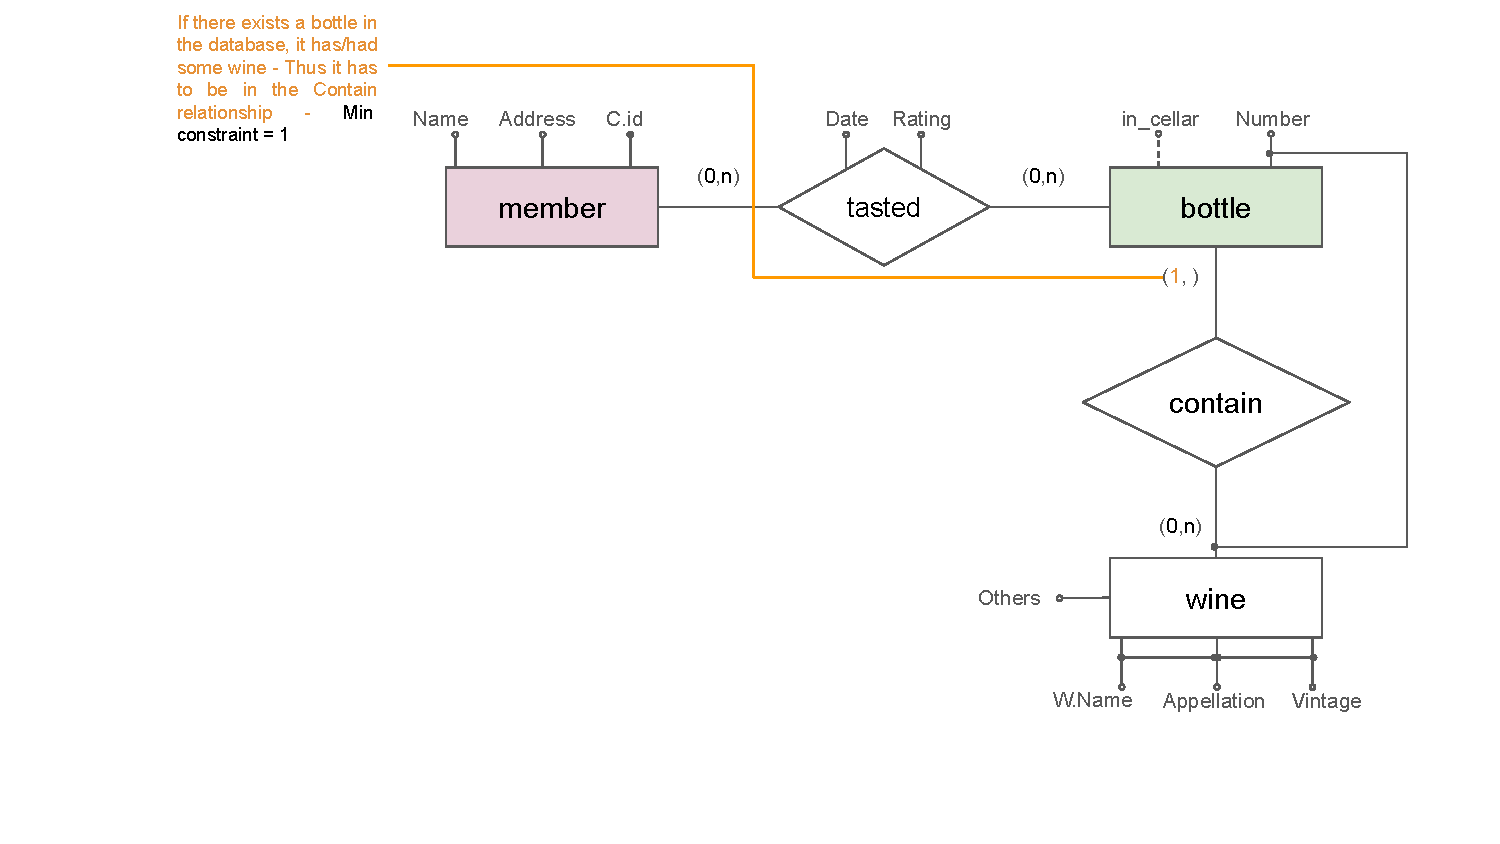
\includegraphics[width=1.1\linewidth]{tut_02_files/17.pdf}
    \end{figure}
\end{frame}

\begin{frame}
    \begin{figure}
        \centering
        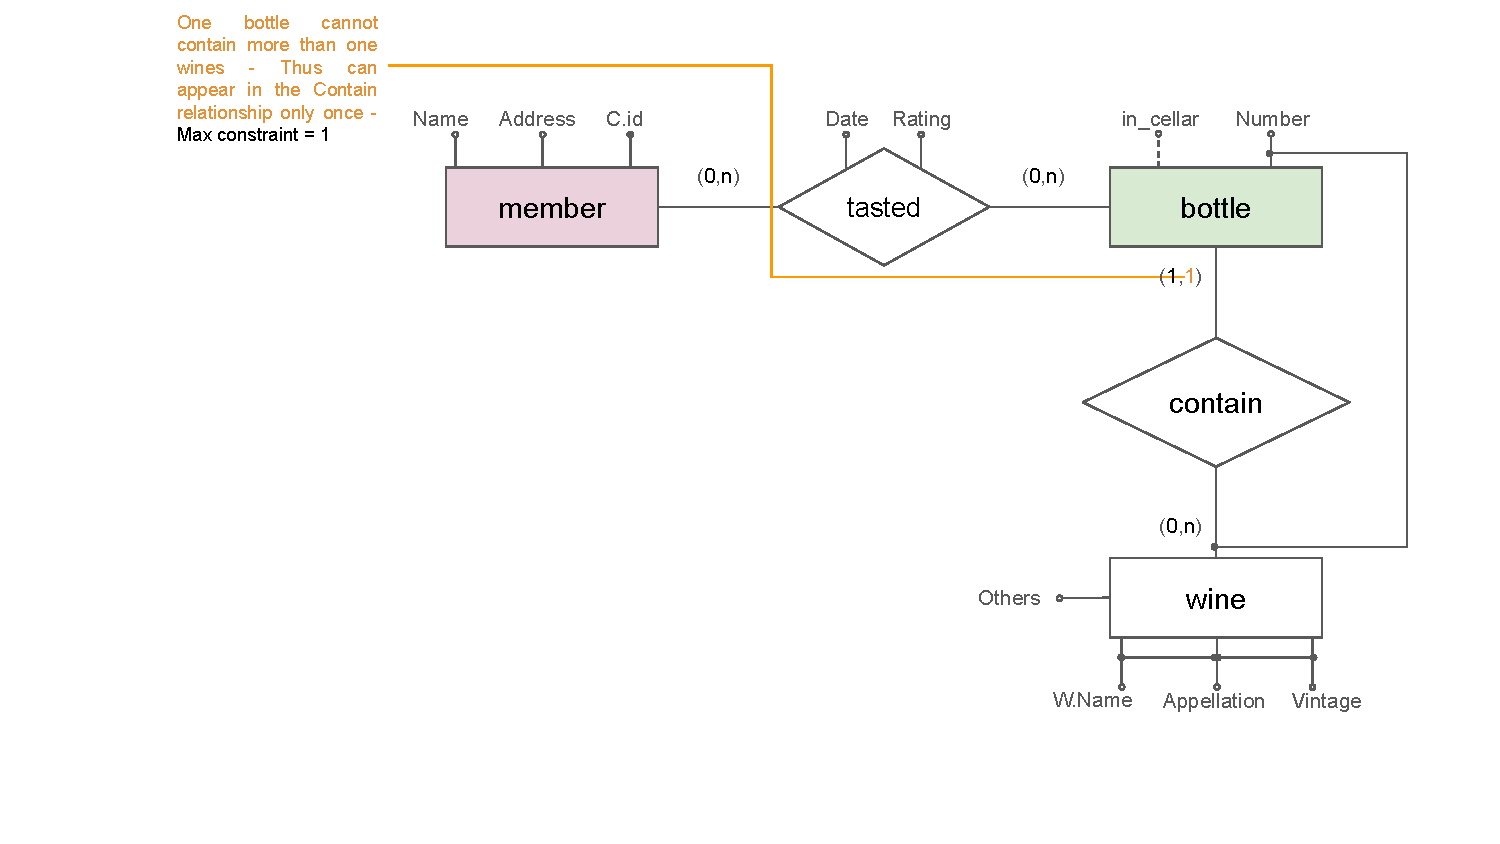
\includegraphics[width=1.1\linewidth]{tut_02_files/18.pdf}
    \end{figure}
\end{frame}

\begin{frame}
    \begin{figure}
        \centering
        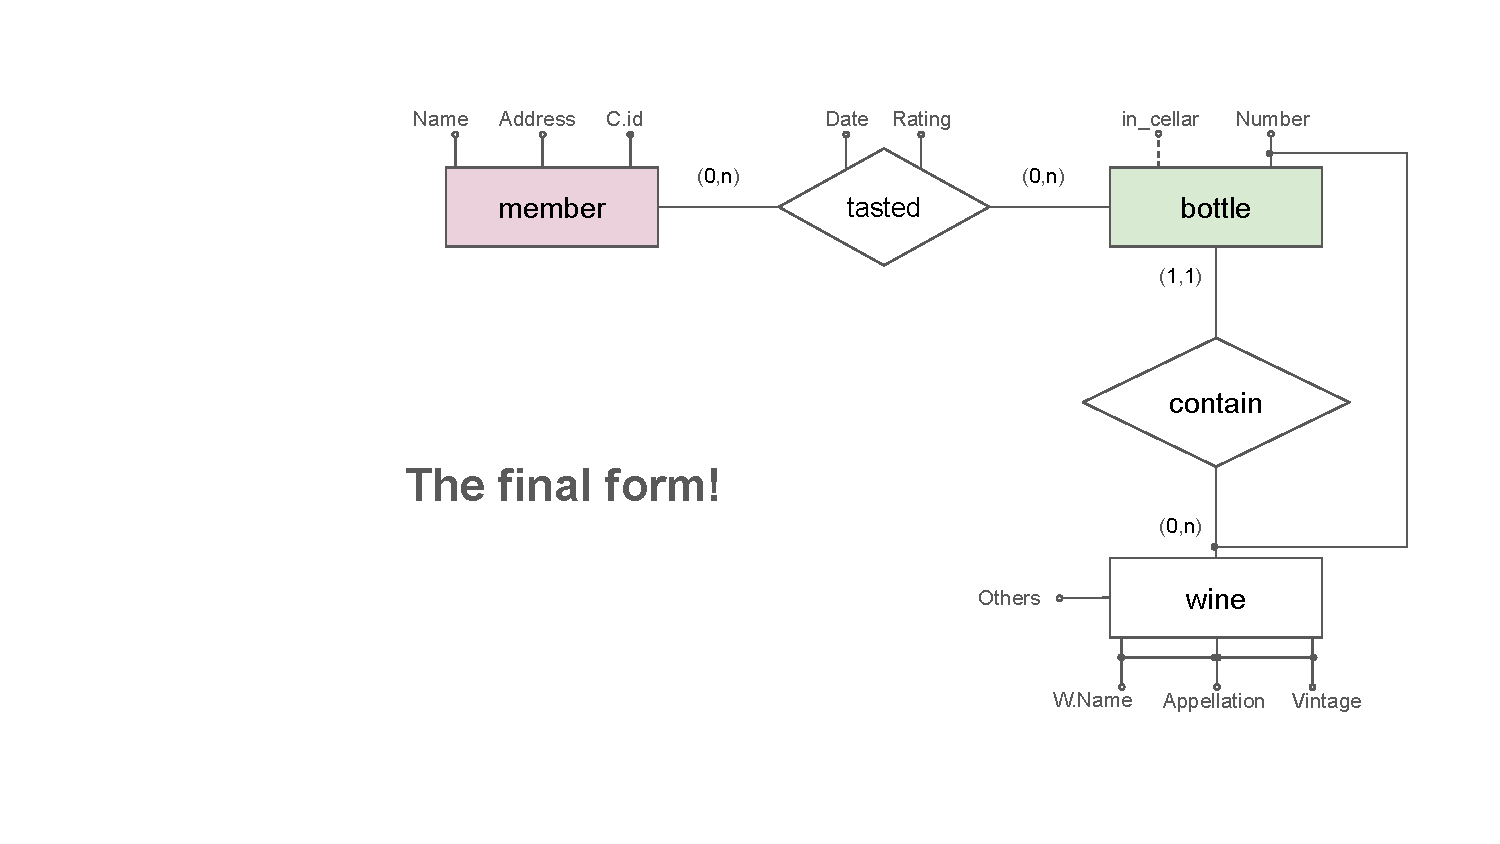
\includegraphics[width=1.1\linewidth]{tut_02_files/19.pdf}
    \end{figure}
\end{frame}

\begin{frame}
    \begin{figure}
        \centering
        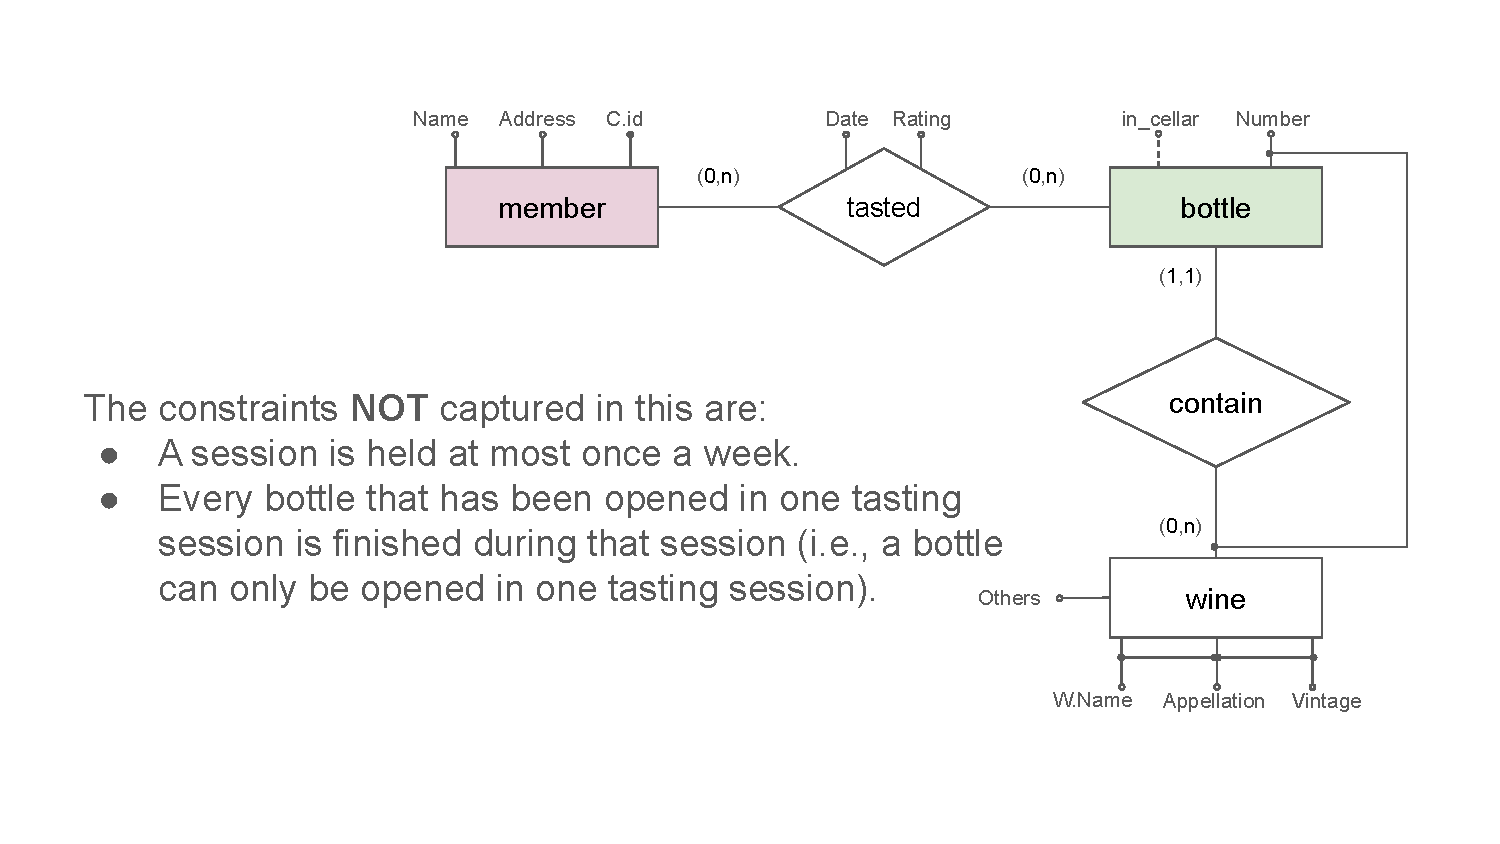
\includegraphics[width=1.1\linewidth]{tut_02_files/20.pdf}
    \end{figure}
\end{frame}

\begin{frame}
    \begin{figure}
        \centering
        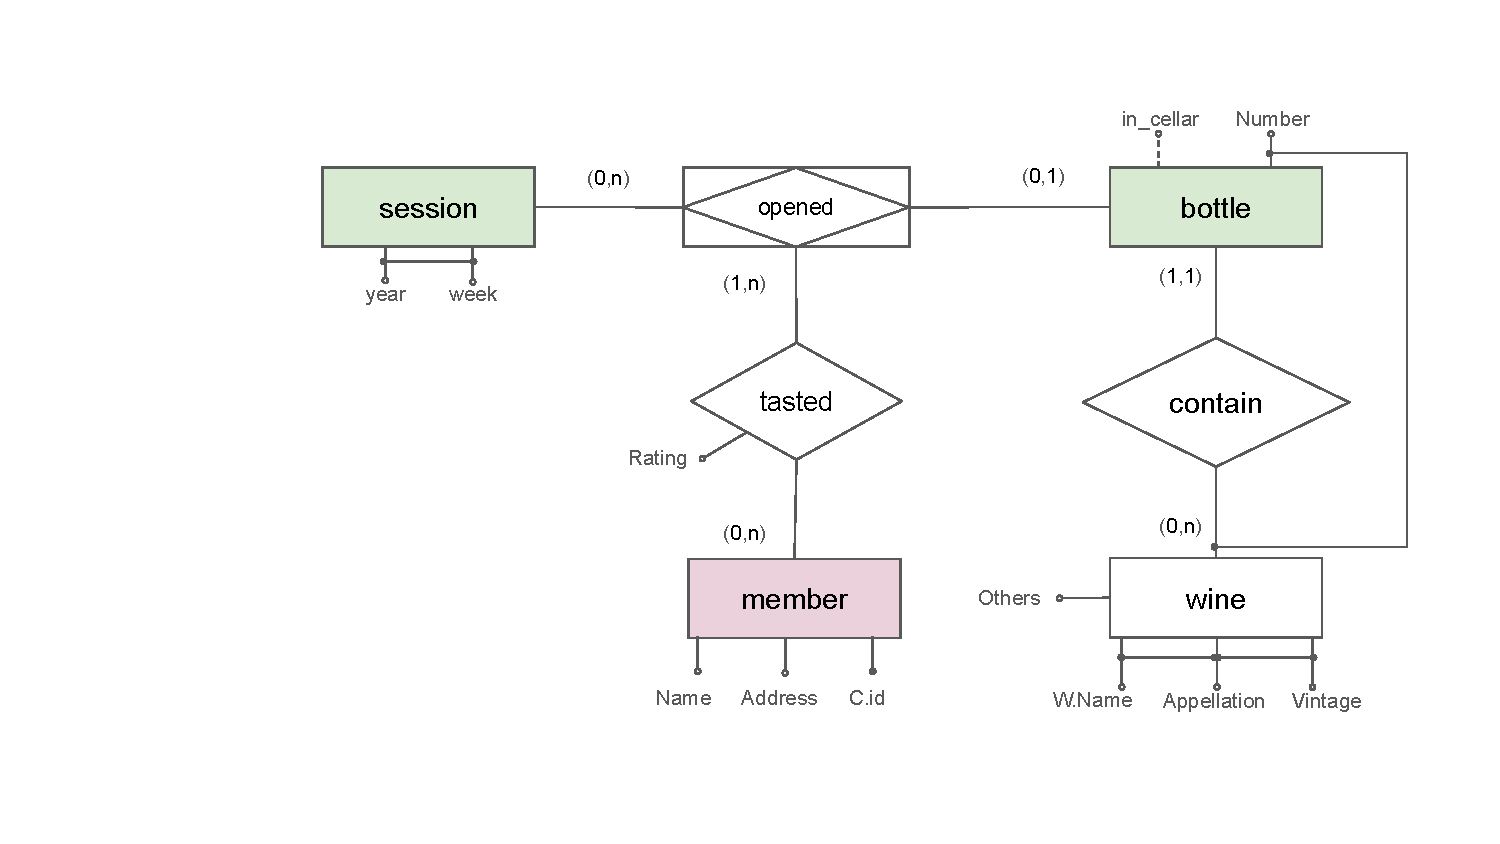
\includegraphics[width=1.1\linewidth]{tut_02_files/21.pdf}
    \end{figure}
\end{frame}

\begin{frame}{Q2. Logical Design}
Translate the final ER diagram (with \texttt{session}, \texttt{open}, and aggregation) into a relational schema.
\begin{itemize}
  \item Strong entities \texttt{member}, \texttt{wine}, \texttt{session}: attributes carry over, entity key becomes the primary key.
  \item Weak entity \texttt{bottle}: primary key = its partial key (\texttt{number}) concatenated with \texttt{wine}'s key.
  \item \texttt{contain} (bottle $\to$ wine, (1,1)): FK on \texttt{bottle}, absorbed into its own row.
  \item \texttt{open} (session $\leftrightarrow$ bottle, bottle side (0,1)): its own table, keyed by \texttt{bottle}.
  \item Aggregated \texttt{taste} (member $\leftrightarrow$ open): FK references \texttt{open}, not \texttt{bottle} directly.
\end{itemize}
\end{frame}

\begin{frame}[fragile]{Q2. Logical Design — \texttt{member} \& \texttt{wine}}
\begin{lstlisting}[language=SQL]
CREATE TABLE member (
  number  CHAR(10) PRIMARY KEY,
  name    VARCHAR(32) NOT NULL,
  address VARCHAR(64) NOT NULL
);

CREATE TABLE wine (
  name            VARCHAR(32),
  appellation     VARCHAR(32),
  vintage         INTEGER,
  alcohol_degree  NUMERIC NOT NULL,
  bottled         VARCHAR(128) NOT NULL,
  certification   VARCHAR(64),
  country         VARCHAR(32) NOT NULL,
  PRIMARY KEY (name, appellation, vintage)
);
\end{lstlisting}
\end{frame}

\begin{frame}[fragile]{Q2. Logical Design — \texttt{session} \& \texttt{bottle}}
\begin{lstlisting}[language=SQL, basicstyle=\ttfamily\scriptsize]
CREATE TABLE session (
  year INTEGER,
  week INTEGER,
  PRIMARY KEY (year, week)
);
CREATE TABLE bottle (
  wine_name   VARCHAR(32),
  appellation VARCHAR(32),
  vintage     INTEGER,
  number      INTEGER CHECK (number > 0),
  PRIMARY KEY (number, wine_name, appellation, vintage),
  FOREIGN KEY (wine_name, appellation, vintage)
    REFERENCES wine (name, appellation, vintage)
);
\end{lstlisting}
\small\textbf{(1,1) on bottle's contain} $\to$ (\texttt{wine\_name, appellation, vintage}) is NOT NULL by construction of the PK.
\end{frame}

\begin{frame}[fragile]{Q2. Logical Design — \texttt{open}}
\begin{lstlisting}[language=SQL, basicstyle=\ttfamily\scriptsize]
CREATE TABLE open (
  wine_name     VARCHAR(32),
  appellation   VARCHAR(32),
  vintage       INTEGER,
  bottle_number INTEGER,
  session_year  INTEGER NOT NULL,
  session_week  INTEGER NOT NULL,
  PRIMARY KEY (bottle_number, wine_name, appellation, vintage),
  FOREIGN KEY (session_year, session_week)
    REFERENCES session (year, week),
  FOREIGN KEY (bottle_number, wine_name, appellation, vintage)
    REFERENCES bottle (number, wine_name, appellation, vintage)
);
\end{lstlisting}
\small\textbf{Bottle (0,1) in \texttt{open}}: a row exists only for bottles that have been opened $\to$ \texttt{open}'s PK = \texttt{bottle}'s key (at most one session per bottle).
\end{frame}

\begin{frame}[fragile]{Q2. Logical Design — \texttt{taste} (aggregate)}
\begin{lstlisting}[language=SQL, basicstyle=\ttfamily\scriptsize]
CREATE TABLE taste (
  wine_name     VARCHAR(32),
  appellation   VARCHAR(32),
  vintage       INTEGER,
  bottle_number INTEGER,
  member        CHAR(10),
  rating        VARCHAR(32) NOT NULL,
  PRIMARY KEY (member, bottle_number, wine_name, appellation, vintage),
  FOREIGN KEY (member) REFERENCES member (number),
  FOREIGN KEY (bottle_number, wine_name, appellation, vintage)
    REFERENCES open (bottle_number, wine_name, appellation, vintage),
  CHECK (rating IN ('very good', 'good', 'average',
                     'mediocre', 'bad', 'very bad'))
);
\end{lstlisting}
\small Referencing \texttt{open} (not \texttt{bottle}) is what the aggregation encodes: a rating is tied to a specific \emph{opening event}, not just to a bottle.
\end{frame}

\begin{frame}
\begin{center}
Questions?\\
Drop a mail at: pratik.karmakar@u.nus.edu
\end{center}
\end{frame}
\end{document}